% Indicate the main file. Must go at the beginning of the file.
% !TEX root = ../main.tex

%----------------------------------------------------------------------------------------
% CHAPTER TEMPLATE
%----------------------------------------------------------------------------------------


\chapter{Planificació}

\label{Planificació}

%----------------------------------------------------------------------------------------
% SECCIÓ 1: Planificació inicial del projecte
%----------------------------------------------------------------------------------------
\section{Planificació inicial del projecte}
A les primeres reunions realitzades amb el tutor es van esbossar quins haurien de ser els passos que s'haurien de seguir per poder complir amb els objectius que plantejats, així i tot, és molt difícil planificar exactament tota la feina que s'ha de realitzar, ja que és difícil estimar el temps que es tarda a fer cada tasca ja sigui per limitacions de la tecnologia usada que poden causar que certes modelitzacions siguin inviables.\\

La planificació inicial susceptible a canvis és la següent:

\begin{itemize}
    \item Adquisició de coneixement sobre l'API de Z3.
    \item Entendre el treball fet per en Sean Patterson veure els seus viewpoints i decidir si se'n podia aprofitar algun.
    \item Implementar mecànica a mecànica del joc al model i avaluar el seu funcionament.
    \item Crear un set d'instàncies per posar a prova el model bàsic.
    \item Analitzar el model actual i fer iteracions amb millors tot analitzant el seu rendiment.
    \item Donat el rendiment valorar si és possible afegir més complexitat al model.
    \item Crear una interfície gràfica per visualitzar les instàncies resoltes.
\end{itemize}

Durant el transcurs del desenvolupament del projecte s'ha seguit la planificació que s'havia pensat a l'inici, però per millor descripció de les tasques, tot seguit què s'ha fet concretament a cada fase i les petites desviacions de la planificació inicial que han sorgit.

\section{Seguiment de la planificació}
\subsection{Ús de l'API de Z3}
A tots els projectes que requereixen l'ús d'una nova tecnologia hi ha una primera fase d'estudi i exercicis. En aquest cas per agafar experiència amb l'ús de l'API de Z3 s'ha seguit la guia Z3 Tutorial \cite{Z3Tutorial} publicada a Google Collaborate, en aquest document es proposen tot d'exercicis, explicacions dels diferents tipus de variables, operadors lògics i funcions que ofereix Z3. Alguns d'aquests exercicis tracten de problemes clàssics com el de les N-reines, Send More Money d'entre altres.\\
Aquesta guia juntament amb la lectura complementària dels punts més importants de la documentació Programming Z3 \cite{Z3Documentation} creada pels contribuïdors del Theorem Prover Z3 des de l'equip de recerca de Microsoft, ha sigut ser essencial per aprendre i assolir una base sòlida de coneixement sobre Z3 per poder començar a plantejar viewpoints i abordar el problema principal.

\subsection{Anàlisi del treball fet a St. Andrews}
Per aquesta fase s'ha fet ús d'un Notebook de Jupyter per poder fer petits experiments sobre els viewpoints explicats al treball Towards Automatic Design of Factorio Blueprints \cite{arxivpaper}. El model creat al paper mencionat s'usa una arquitectura multinivell on se secciona el problema en diferents fases, aquesta decisió es veu influenciada per la limitació de PDDL de modelar variables contínues i a les millores del model proposen unificar el model per ajudar al solver a fer propagació i no comprovar solucions redundants.\\
Per aquest motiu la majoria del plantejament realitzat al paper no s'ha pogut usar. En un dels nivells de l'arquitectura que es comenta al paper, s'explica la representació que es fa per modelar les rutes que les cintes de transport segueixen, concretament es parla de la representació incremental i direccional, les quals s'han usat al model desenvolupat en aquest projecte. Aquesta representació s'ha implementat de manera temporal al Notebook mencionat per analitzar el rendiment i escalabilitat de la modelització.\\
Finalment, del paper també s'han extret algunes les mecàniques principals (rutes, tipus d'objectes i quantitat d'objectes) que conformen part del model del projecte.

\subsection{Implementació del model bàsic}
El modelatge i implementació de les restriccions ha estat la que més temps ha dut completar, ja que moltes de les modelitzacions que codifiquen les mecàniques bàsiques del joc han requerit ser modificades múltiples vegades. Concretament, una de les parts més importants del model (quantitat d'objectes), ha passat per tres iteracions fins que el seu comportament ha sigut el desitjat.\\
En aquesta fase s'han implementat totes les restriccions necessàries per crear un model base completament funcional sobre el qual, retocar alguns comportaments, implementar optimitzacions i fer una anàlisi del rendiment per veure si el projecte avança per bon camí i si realment s'està fent una aportació valuosa al camp de la lògica i la intel·ligència artificial.

\subsection{Creació d'instàncies}
Amb la base del model implementada cal un set d'instàncies per poder veure el comportament del model, fer proves, descobrir si hi ha algun error en la implementació i comprovar el rendiment.\\
Inicialment, es volien crear les instàncies manualment, buscant les receptes que les fàbriques poden usar, seleccionant les entrades i sortides dels materials, els tipus... aquesta manera és molt ineficient a causa de l'enorme quantitat de receptes que el joc conté, com aquestes receptes poden requerir altres receptes, els materials que aquestes impliquen i com és de poc intuïtiu introduir coordenades d'una graella sense poder tenir una representació gràfica per ubicar on està cada casella. Així que aquesta fase de la planificació no només s'han generat totes les instàncies necessàries sinó que també s'ha hagut de desenvolupar una eina per poder-les generar de manera automàtica a partir d'una interfície gràfica fàcil d'usar.\\
Les instàncies estan enfocades a posar a prova diferents aspectes del model, ja sigui perquè requereixen moltes receptes, l'espai és reduït o les receptes requereixen molts o poc materials d'entrada. També s'ha jugat amb les ràtios d'entrada i sortida de les receptes.

\subsection{Aplicar millores sobre el model base}
Després d'analitzar el model base s'ha fet una reunió amb el tutor on ha sorgit una optimització que simplifica força el model. Durant la implementació de l'optimització també han sorgit un upper i lower bound que han ajudat força. Finalment, hi ha hagut 3 canvis respecte al comportament del model per replicar amb millor precisió el funcionament real del joc.\\
Amb aquestes millores aplicades, s'ha fet un script en Python que conté el set d'instàncies usat per fer proves sobre el rendiment i s'ha deixat l'ordinador resoldre-les amb un timeout de 1800 segons. Tenint en compte que hi ha tres millores substancials i s'han fet optimitzacions seguint tres criteris diferents, el procés de resoldre instàncies ha durat unes tres setmanes.

\subsection{Visualització de les instàncies resoltes}
Finalment, amb el model completament finalitzat, s'han dedicat dues setmanes i mitja de treball diària en implementar l'apartat de la web encarregat de visualitzar les instàncies de manera gràfica. El desenvolupament s'ha separat en dues parts principals. Primer el pre procés de les dades d'una instància resolta, per ser guardades de manera còmoda per mes tard ser llegides i mostrades per pantalla, aquest pre procés implica saber quines imatges s'han de mostrar per casella, saber la informació que ha de contenir cada casella en funció del seu tipus...\\
La segona part tracta de la implementació de la part purament gràfica, és a dir les mides de les imatges, l'orde de dibuixat de les imatges, creació i modificació d'algunes imatges, disseny de la part HTML que mostra les dades, entra d'altres tasques.\\
A banda també hi va haver una petita fase de disseny abans de la implementació.

\subsection{Redacció de la memòria}
Una de les parts més importants del projecte és redactar una bona memòria, encara que no sembli que hagi d'ocupar gran part del projecte, ha sigut una de les tasques que més hores ha comportat a causa de la quantitat de coses que s'han d'explicar, les quals han comportat la creació de gràfics, exemples, formalitzacions, complicació de dades dels experiments... Que són moltes petites tasques que acumulen molta feina. Com des d'un bon principi se sabia que la redacció de la memòria és un dels apartats amb més feina, s'ha anat redactant al llarg del projecte els apartats més feixucs del disseny i desenvolupament del model juntament amb alguns dels apartats dels conceptes previs, els quals han alleugerit la feina al final del projecte.

\begin{sidewaysfigure}
    \centering
    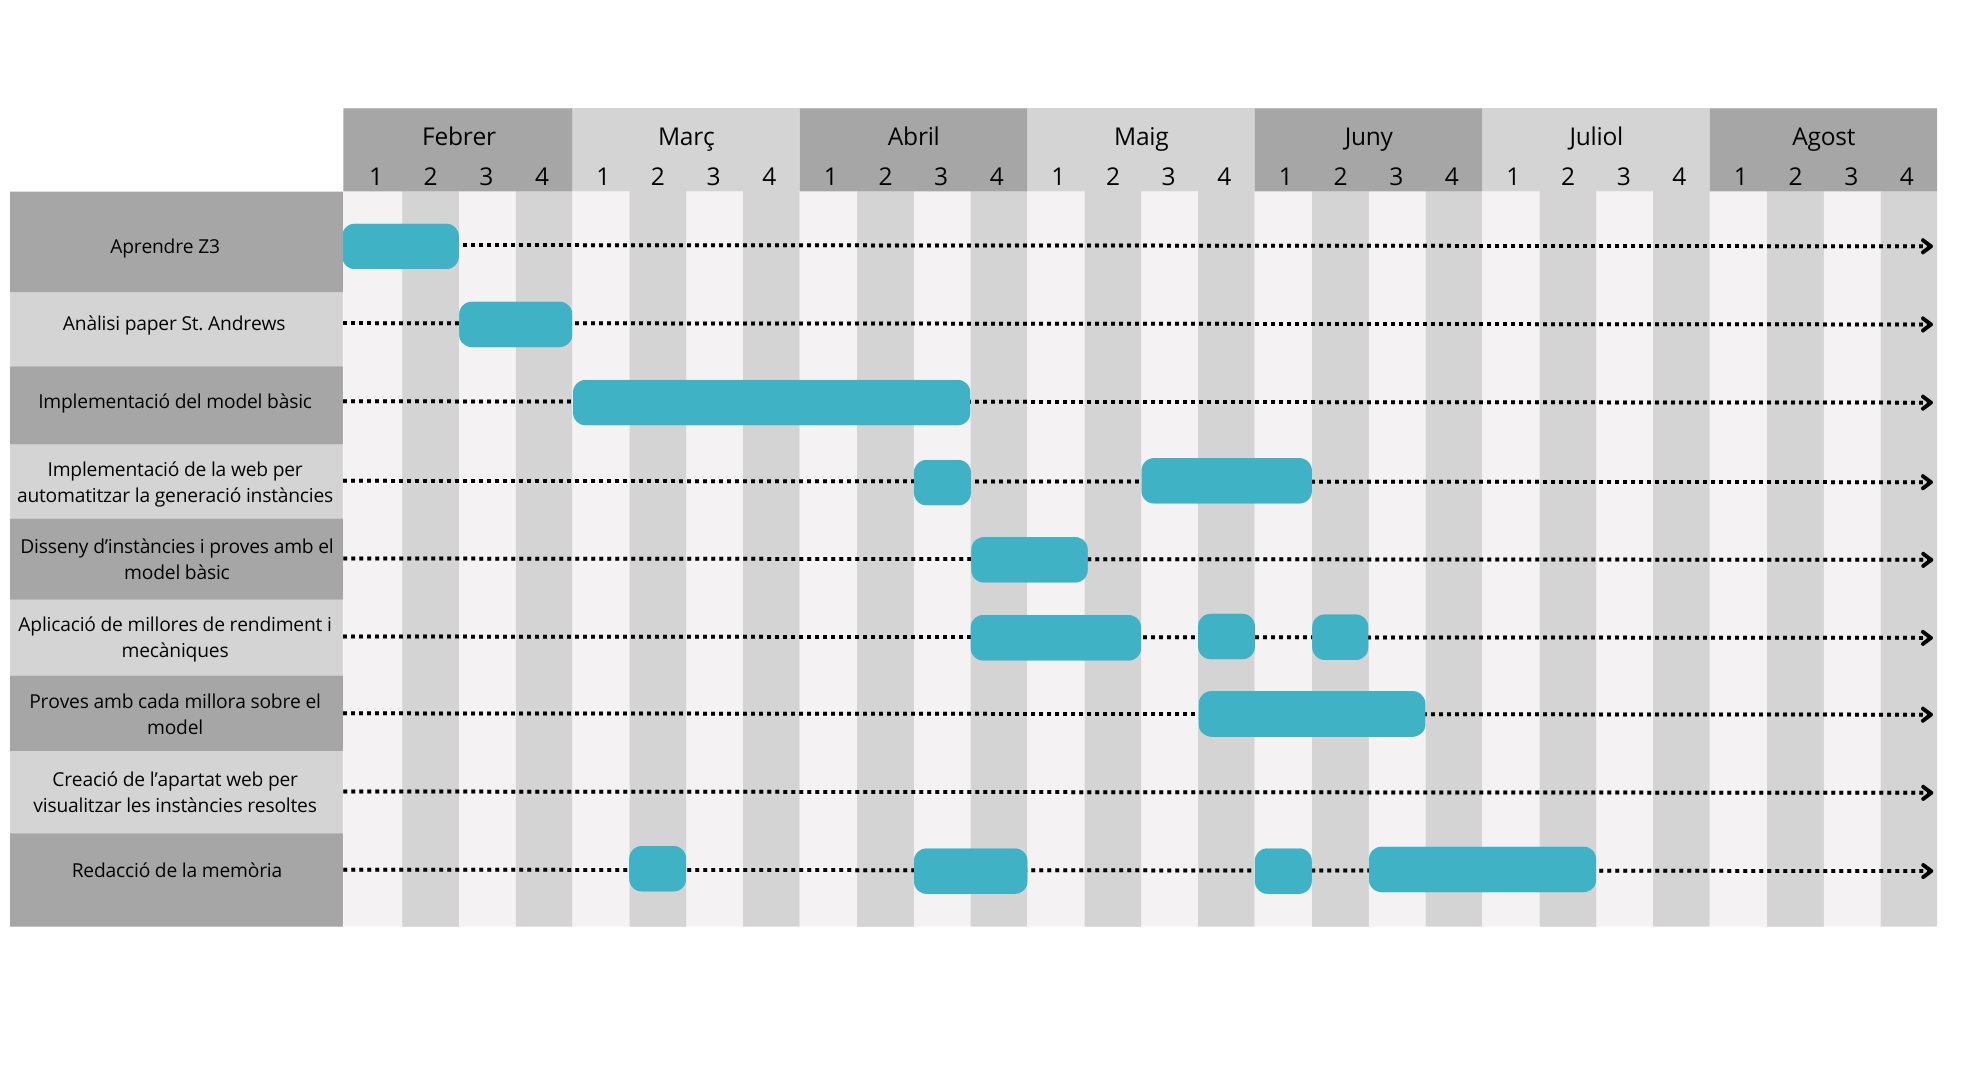
\includegraphics[width=1\linewidth]{Figures//miscelaneous/diagrama-grantt.png}
    \caption{Diagrama de Grantt del desenvolupament del projecte}
    \label{fig:diagrama-grantt}
\end{sidewaysfigure}
